\documentclass[a4paper]{article}
\usepackage{graphicx}

\title{Ocframe Manual  \\ {\large  Structural Analysis functions of the Mechanics package}}
\author{Johan Beke}

\begin{document}

\maketitle

\tableofcontents
% for F in *.m; do octave -q --eval "get_help_text_from_file(\"$F\")"; done > output.texi
% for F in *.m; do octave -q --eval "disp(get_help_text_from_file(\"$F\"))"; done > ref.texi ; makeinfo --plaintext ref.texi > ref.txt

\section{Introduction}
	\begin{sloppypar}
	The structural analysis functions of the \emph{Mechanics} packages where written during a FEM course. The following posibilities are in the package:
		\begin{itemize}
			\item The analysis of 2D frames with rigid connections with the function {\emph{SolveFrame}}.
			The solutions for the reaction forces, displacements and member end forces are given.
			\item Solution of multiple load cases at once with the function \emph{SolveFrameCases}
			\item A plot of the frame, with nodal displacements if needed, with the function \emph{PlotFrame}. The nodes and members are numbered.
			\item Calculation the member internal forces for each member with the function \emph{MSNForces}
			\item Plot of the internal member forces diagram with the function \emph{PlotDiagrams}
		\end{itemize}
	\end{sloppypar}
\section{Conventions}
	\subsection{Units}
		\begin{sloppypar}
		The user can use any units as long as they are consistent. So if the forces are provided 
		in kN, kN/m and kNm, the geometry and member properties must be in similar units (m, m$^2$, m$^4$ and kN/m$^2$). 
		\end{sloppypar}
	\subsection{Global and local axis}
		\begin{sloppypar}
		For the nodes and the members, care must be taken for the axes. 
		The following images show the used coordinate systems (figure \ref{fig:axis.png}) 
		and the conventions for the member forces (figure \ref{fig:dist.png} and \ref{fig:point.png}). 
		The local axes are always from the near node to the far node.
		\end{sloppypar}
		\begin{figure}[h]
			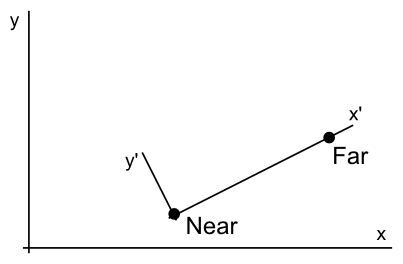
\includegraphics[width=0.50\linewidth]{axes.png}
			\caption{Local and global axis convention}
			\label{fig:axis.png}
		\end{figure}
		\begin{figure}[tb]
			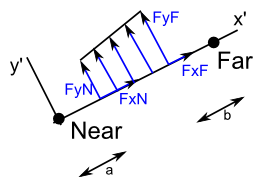
\includegraphics[width=0.50\linewidth]{dist.png}
			\caption{Conventions for a distributed load on a member}
			\label{fig:dist.png}
		\end{figure}
		\begin{figure}[tb]
			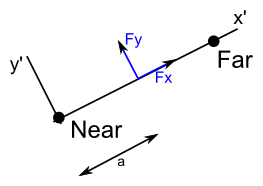
\includegraphics[width=0.50\linewidth]{point.png}
			\caption{Conventions for a point load on a member}
			\label{fig:point.png}
		\end{figure}
		\begin{figure}[tb]
			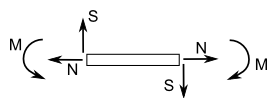
\includegraphics[width=0.50\linewidth]{sign_conv.png}
			\caption{Sign conventions for internal forces}
			\label{fig:sign_conv.png}
		\end{figure}

\newpage
\section{Example}
	\begin{sloppypar}
	An example will clarify the usage of the different functions.
	\end{sloppypar}
	\subsection{Forces and geometry}
	
		\begin{figure}[h]
			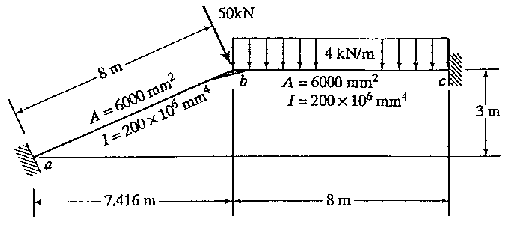
\includegraphics[width=0.75\linewidth]{example5_7.png}
			\caption{Example frame}
			\label{fig:example_frame}
		\end{figure}
		
		\begin{sloppypar}
			An example frame, which was taken from the book Matrix Structural
			Analysis, is shown in figure \ref{fig:example_frame}. 
			The following code snippet is used to enter the geometry:
		\end{sloppypar}
		
		\begin{verbatim}
joints=[0,0,1,1,1;
		7.416,3,0,0,0;
		8+7.416,3,1,1,1];
# first cells of each row are the x and y coordinates
# next cells are the x, y and z constraints. 
# node 1 and 3 are fully fixed, node 2 is free

# member data
E = 210.0e3; # N/mm^2 = MPa
A = 6000;# mm^2
I = 200.0e6;# mm^4

# convert units to kN and m
E = E*10^3;
A = A*(10^-3)^2;
I = I*(10^-3)^4,

#connectivity data
members=[1,2,E,I,A;
		2,3,E,I,A];
		\end{verbatim}
		
	\subsection{Loads}
		\begin{sloppypar}
			The following code snippet is used to enter the loads:
		\end{sloppypar}
		\begin{verbatim}
			# point load on node 2
			# Fx = 18.75 kN
			# Fy = -46.35 kN
			# Mz = 0 kNm
			nodeloads=[2, 18.75,-46.35, 0.0];
			
			loc = 1;
			glob = 0;
			
			# distributed load on member 2
			# Fx = 0 kN/m 
			# Fy = -4 kN/m
			# same for the end of the load
			# a = b = 0 m  load on full span
			# local load
			dist=[2,0,-4.0,0,-4.0,0.0,0.0,loc];
			#no point loads on members
			point=[];
		\end{verbatim}

	\subsection{Solutions}
		\begin{sloppypar}
			The following code snippet is used to find the basic solution:
		\end{sloppypar}
		\begin{verbatim}
			[P,D,MemF]=SolveFrame(joints,members,nodeloads,dist,point);
		\end{verbatim}
		\begin{sloppypar}
			The basic solution are the reactions, the displacements and the member end forces:
		\end{sloppypar}
		\begin{verbatim}
			P =

			   130.497    55.677    13.374
				   NaN       NaN       NaN
			  -149.247    22.673   -45.356

			D =

			   0.0000000   0.0000000   0.0000000
			   0.0009476  -0.0047441  -0.0005088
			   0.0000000   0.0000000   0.0000000

			MemF =

			   141.8530     2.6758    13.3742  -141.8530    -2.6758     8.0315
			   149.2473     9.3266    -8.0315  -149.2473    22.6734   -45.3557
		\end{verbatim}
		\begin{sloppypar}
			Each row of the reaction matrix (matrix P in this case) corresponds to the node. (First row to first node, etc.).
			The columns are R$_x$, R$_y$ and M$_z$. For node 1 the reactions are thus: R$_x$ = 130.497 kN, R$_y$ = 55.677 kN and M$_z$ = 13.374 kNm.
			In case of a free component without reactions, the value is represented by NaN.\\
			The same convention holds for the displacement matrix (matrix D in this case). For node 2 the displacements are thus:
			x = 0.0009476 m, y = -0.0047441 m and rotation = -0.0005088 rad.\\
			A similar principle holds for the member-end-forces. Each row corresponds to the element. The columns are: F$_x$, F$_y$, M$_z$, F$_x$, F$_y$ and M$_z$ where 
			the first three components are for the first node and the last three components are for the last node.
			
		\end{sloppypar}

\newpage
\section{Function reference}
		\begin{verbatim}
 -- Function File: [X, M, S, N] =  MSNForces (JOINTS, MEMBERS, DIST,
          POINT, MEMF, MEMBERNUM, DIVISIONS)
     This function returns the internal forces of a member for each
     position x. The member  is divided in 20 subelements if the
     argument is not given. The used sign convention is displayed in
     the help file.

     Input parameters are similar as with SolveFrame and PlotFrame with
     extra arguments:

     membernum = Number of the member to calculate     divisions =
     Number of divisions for the member


 -- Function File:  ocframe_ex1 ()
     Example of a planar frame.


 -- Function File:  ocframe_ex2 ()
     Example of a beam.


 -- Function File:  ocframe_ex3 ()
     Example of a planar frame.


 -- Function File:  ocframe_exLC ()
     Example of a beam with generation of eurocode ULS  load cases


 -- Function File:  ocframe_railwaybridge ()
     Example taken from a real railwaybridge.


 -- Function File:  ocframe_tests ()
     Various tests for the entire package.   Test 1, 2 & 3 are simple
     beams (tested for reactions and internal forces)  Test 4 & 5 are
     frames (tested for reactions)

 -- Function File:  PlotDiagrams (JOINTS, MEMBERS, DIST, POINT, MEMF,
          DIAGRAM, DIVISIONS, SCALE)
     This function plots the internal forces for all members. The force
     to be plotted can be selected with DIAGRAM  which will be "M", "S"
     or "N" for the moment, shear or normal forces.

     Input parameters are similar as with SolveFrame and PlotFrame.

 -- Function File:  PlotFrame (JOINTS, MEMBERS, D, FACTOR)
     Plots a 2D frame (with displacements if needed) using  the
     following input parameters:

     joints = [x , y, constraints ; ...]

     constraints=[x , y, rotation] free=0, supported=1

     members = [nodeN, nodeF, E, I, A; ...]

     	  Optional arguments:

     D = [x,y,rotation;...] Displacements as returned by SolveFrame

     factor= Scaling factor for the discplacements (default: 10)


 -- Function File: [RESULTS] = SolveFrameCases (JOINTS, MEMBERS,
          LOADCASES)
     Solves a 2D frame with the matrix displacement method for  the
     following input parameters:

     joints = [x , y, constraints ; ...]

     constraints=[x , y, rotation] free=0, supported=1

     members = [nodeN, nodeF, E, I, A; ...]

     loadcases is a struct array with for each loadcase the fields

     - nodeloads = [node, Fx, Fy, Mz; ...]

     - dist = [membernum,FxN,FyN,FxF,FyF,a,b,local ; ...]

     - point = [membernum,Fx,Fy,a,local; ...]

     input is as for the function SolveFrame.

     Output is a struct array with the fields: Displacements, Reactions
     and MemF

     (output formated as for the function SolveFrame.)

 -- Function File: [REACTIONS, DISPLACEMENTS, MEMF] =  SolveFrame
          (JOINTS, MEMBERS, NODELOADS, DIST, POINT)
     Solves a 2D frame with the matrix displacement method for  the
     following input parameters:

     joints = [x , y, constraints ; ...]

     constraints=[x , y, rotation] free=0, supported=1

     members = [nodeN, nodeF, E, I, A; ...]

     nodeloads = [node, Fx, Fy, Mz; ...]

     loads on members:

     dist = [membernum,FxN,FyN,FxF,FyF,a,b,local ; ...] for distributed
     loads     where FxN and FyN are the loads on distance a from the
     near node     (same with far node and distance b)     local=1 if
     loads are on local axis, 0 if global

     point = [membernum,Fx,Fy,a,local; ...]      where Fx and Fy are
     the loads on distance a from the node near     local=1 if loads
     are on local axis, 0 if global

     Output is formated as follows (rownumber corresponds to     node
     or member number):

     Reactions = [Fx,Fy,Mz;...] where NaN if it was a non supported dof

     Displacements = [x,y,rotation;...]

     MemF = [FxN, FyN, MzN, FxF, FyF, MzF; ...]
	\end{verbatim}
\end{document}
